%TODO: the fact that we we do not use tree structure violates "the lore". I have never seen AHP algorithms that would be
%implemented in this way.

%TODO: MAYBE: I have managed to formulate formal requirements for the graph that we use. What
%if I write them as well? I define there a notion of level (to some extent), and reveal constraints that make the
%recursive approach applicable.

%TODO: Constraints. We do not:
% 1. Delve into an agent's reasoning process;
% 2. Imply any particular structure of the graph;
% 3. Imply any particular implementation of an agent, neither its reasoning process (although we model that in our
%    "implementation" section)
 %4. What triggers a decision making
% 5. Although we use AHP, we do not emphasize use of this particular one
% 6. The nature of the actions
% 7. Who adjusts the strategy weights

% TODO: plan
% -- hierarchy of preferences
% ?? formal description of the graph. Definitions: levels
% -- separation of responsibilities, the actual approach to simulation
% -- definitions: aspects (contexts), levels
% -- fusion of tactical decisions up to the general objective (moving up the contexts)
% -- using AHP for this
% -- the recursive algorithm implementing the idea

In order to incorporate both strategic and tactical objectives into the decision making process we propose to represent
the latter as a result of decomposing strategic ones. By that, we do not necessarily mean that tactical objectives have
to be mutually exclusive components, represent dependencies or certain milestones, although that is probably an option.
It implies that any lower-level objective may be a part of two or more higher-level ones. This decomposition can be
represented as a hierarchy of preferences or a weighted preference graph (Figure \ref{fig:prefgraph-concept-shared}).
%TODO: ref figure
%TODO: ref preference graph

\begin{figure}[hbt!]
    \centering
    \begin{subfigure}{.45\linewidth}
        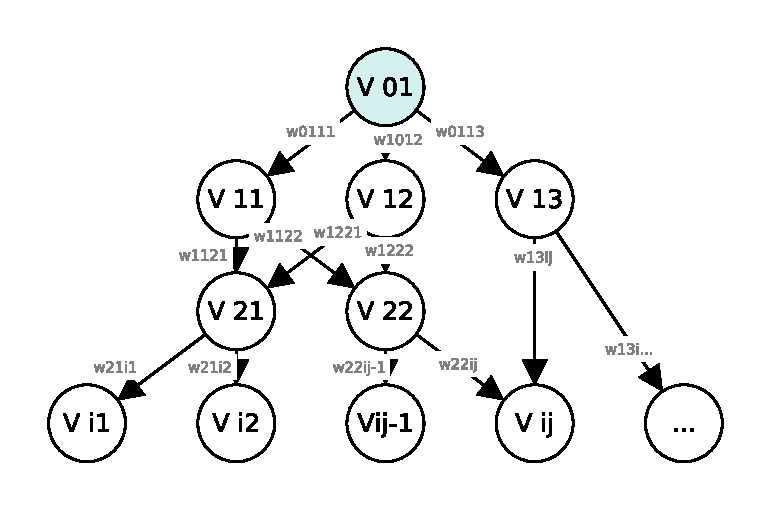
\includegraphics[width=\textwidth]{prefgraph-concept.eps}
        \caption{Shared graph}\label{fig:prefgraph-concept-shared}
    \end{subfigure}
    \begin{subfigure}{.45\linewidth}
        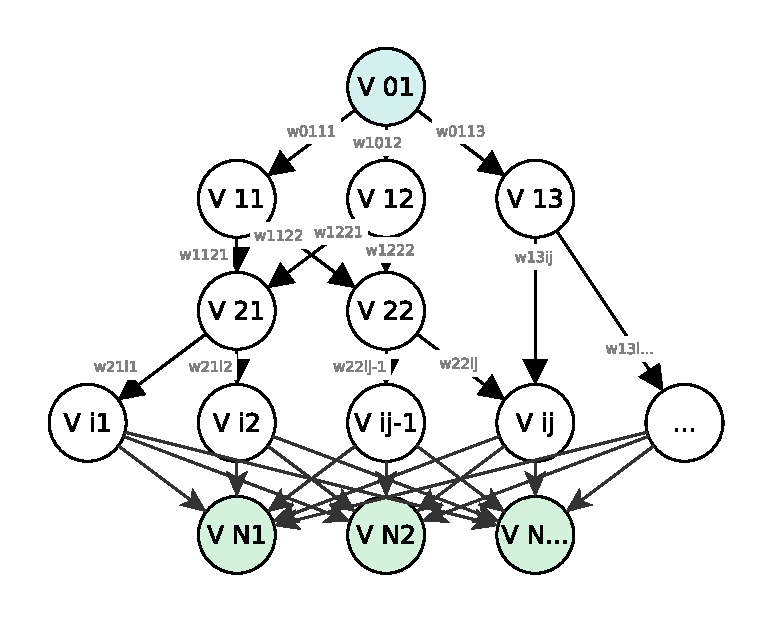
\includegraphics[width=\textwidth]{prefgraph-concept-extended.eps}
        \caption{Local graph}\label{fig:prefgraph-concept-local}
    \end{subfigure}

    \caption{\small An example of a preference graph}
    \label{fig:prefgraph-concept}
\end{figure}

However, this graph (Figure \ref{fig:prefgraph-concept-shared}) is only a part of a preference graph as it lacks
alternatives. Adding alternatives will give us the full-fledged preference graph (Figure
\ref{fig:prefgraph-concept-local}). For reasons that will soon become obvious we call the graph in Figure
\ref{fig:prefgraph-concept-shared} "shared" and the one in Figure \ref{fig:prefgraph-concept-local} "local".

With use of the weighted preference graph, a decision is made through calculating a vector of weights representing
valuability of each of the alternatives $\fnmalts$ \textit{in the context of} node $\fnmroot$ which is
achieved through iterative calculations involving intermediate nodes $\fnmnode i j$, edges, and weights.

Changing weights of any of the preference graph's edges will change the resulting vector calculated for the alternatives
$\fnmalts$. This fact is at the core of the approach we propose which reads as follows:

\begin{itemize}
    \item The structure of neither shared nor local graphs gets changed during the simulation;
    \item Weights connecting the alternatives $\fnmalts$ and those connecting the node $\fnmroot$ are the only ones that
        change during the simulation;
    \item Every agent may read the shared graph (Figure \ref{fig:prefgraph-concept-shared}), its weights and structure;
    \item Every agent has a predefined set of \textit{actions} assigned to it specifically;
    \item Every agent has to select an action which it will perform for a certain timespan, therefore, every action is
        mapped to the preference graph;
    \item Those alternatives plus the shared graph form the local preference graph only visible for this agent (hence
        the name "local");
    \item Before every decision making iteration, the agent assesses alternatives $\fnmalts$ \textit{in the contexts} of
        aspects $ \fnmasps{N-1} $ using its means of local tactical assessment. Then having all the intermediate weights
        it assessess them \textit{in the context of} node $\fnmroot$. The action having the highest weight in the
        resulting vector gets selected for the execution;
    \item In parallel, some entity adjusts weights connecting the node $\fnmroot$ which we interpret as setting
        strategic objectives.
\end{itemize}

In essense we have 2 classes of entities namely a coordinator and an executor. The coordinator changes the high-most
level weights of the shared graph visible to every agent, therefore, influences decisions of the latter. At the same
time agents perform local situation assessments for their actions using their local graphs which are extensions over the
dynamically changing shared one. Changes in the shared graph get fetched and used in an individual agent's reasoning
process.

Despite the fact that necessity to adjust strategic objectives by tweaking high-level weights implies that there should be some entity that does so, we do not elaborate on its implementation.
Neither do we reveal how exactly agents' tactical reasoning processes are implemented, what are the rules of decomposing an ultimate goal that the swarm pursuits, what triggers a decision making process, and for how long an agent executes an action.
Those are details of a particular implementation which should be formulated separately with all the technical limitations, requirements, and subject area features taken into account.

% To enrich the semantics of the decomposition process, we propose to not to limit it by just one iteration.
